% Chapter 1

\chapter{Machine learning} % Main chapter title

\label{Chapter2} % Change X to a consecutive number; for referencing this chapter elsewhere, use \ref{ChapterX}
\section{What is machine learning}
Machine learning is a subfield of Computer Science. It is a type of Artificial Intelligence which allows programs to learn and find patterns within data. \cite{coursera} \\
\\
Machine learning explores algorithms that can learn from and make predictions on data. These algorithms are called machine learning algorithms. A machine learning algorithm has to learn before it can be used to make predictions on data. \textbf{Learning} means that the algorithm has to be shown several examples of data and what the correct predictions for these examples would be. The amount of examples that have to be shown to the algorithm can be within the range of several thousands. \\
\\
Once the machine learning algorithm has learned from the data, it can be used to make predictions on other data. For example, machine learning can be used in order to watch the heartrate of patients at a hospital. During the learning phase, the machine learning algorithm is shown the heartrate of a patient and  the current time. After learning is done, the machine learning algorithm can predict what the heartrate of that patient should be based on the current time. This can be used to determine whether the patients heartrate is normal by comparing the predicted heartrate and the real heartrate.\\
\\
There are two classes of machine learning algorithms. There is \textbf{supervised} learning and \textbf{unsupervised} learning. Supervised learning is trained using labeled data. Labeled data is data which consists of input data and the corresponding output data. Unsupervised learning uses unlabeled data. The data used to train machine learning algorithms is called a \textbf{training set}.\\
\\
Supervised learning is the type of learning when the data presented to the learning algorithm is labeled. This means that the user of the learning algorithm can already make distinctions within the presented data. This is useful for regression or classification problems. Regression is explained in Section~\ref{regression} and Classification is explained in Section~\ref{classification}. \\
\\
Unsupervised learning is the type of learning when the data presented to the learning algorithm is unlabeled. The learning algorithm has to find structure in the given data. \\
\\ 
A \textbf{training sample} is a data point in an available training set that is used in a predictive modeling task. For example, if machine learning is applied to spam filtering, the training set is a collection of emails, some of which are spam emails. A training sample would be a single email. Alternative names are a training example or training instance. \\
\\
Machine learning is applied for predictive modeling. In predictive modeling, a particular process or event is modeled. Using a training set, the model tries to learn or approximate a particular function that, for example, lets us distinguish spam from non-spam email. This function is called the target function. The function the model makes to approximate the target function is called the \textbf{hypothesis}. \\
\\
To model the particular process or event, one or more \textbf{features} are extracted. A feature is an individual property. All features combined define the model of the particular process or event. In the example of mails, a feature could be the textbody, or it could be the sender of the email. It could even be individual characters which appear in the email. Which features are chosen is completely dependent on which problem is being solved. \\\\
This chapter gives an introduction to the mathematical background of supervised machine learning. It starts with lineair regression which is a simple category of machine learning algorithms. The principles behind lineair regression are the same as for other machine learning algorithms. Afterwards logistic regression is used to explain how classification works within machine learning. It begins by explaining what exactly the hypothesis is and how it can be constructed. \cite{courseraLectures}
\section{Lineair Regression}
\label{regression}
Lineair regression is a statistical approach to model the relationship between an "output" value $y$ and one or more "input" values $x_1...x_n$. The "input" values are called features. It belongs to the category of supervised learning. An example of this can be seen in Figure~\ref{fig:regression}. The black dots represent the data to be modeled. The blue line is the model. This example only has one "input" value. This specific case of regression is called simple linear regression. \cite{scikit-regression}. 

\subsection{Hypothesis}
Machine learning relies heavily on a hypothesis which is given the notation $H_0(x)$ in equations. This is a function that transforms a given input to the machine learning algorithm into the required output. It is a function that tries to model the target function, it tries to give a function which fits the input data. The input are features, denoted by $x$.  The values for $\theta$ are unknown values. These values are chosen during the training of the machine learning algorithm and determine how accurate the algorithm is. When only one feature is considered, a hypothesis is a function of the form \cite{stanford}: 
\begin{align}
H_0(x) = \theta_0 + \theta_1 * x 
\end{align}
For example, we could use the grades of high school students to predict their chance of success at university. This is shown in Figure~\ref{fig:regression}. The $x-axis$ represents the grades (on a scale from 0 to 10) for students and the $y-axis$ is the chance of success. Given is input data (the black points) and from that data a hypothesis (the blue line) is constructed. \\\\
The hypothesis function can be generalised for $N$ features. It generally has the form:
\begin{align}
H_0(x) = \theta_0x_0 + \theta_1x_1 + ... + \theta_nx_n
\end{align}
$x_0$ always has the value 1. The $\theta$ values and the $x$ values can be represented using vectors. Now the hypothesis function can be written in a more convenient way:
\begin{align}
\label{hypothesisfunc}
H_0(x) = \theta^TX = [\theta_1, \theta_2, ..., \theta_n]^T [x_0, x_1, ..., x_n]
\end{align}

\begin{figure}[H]
\centering
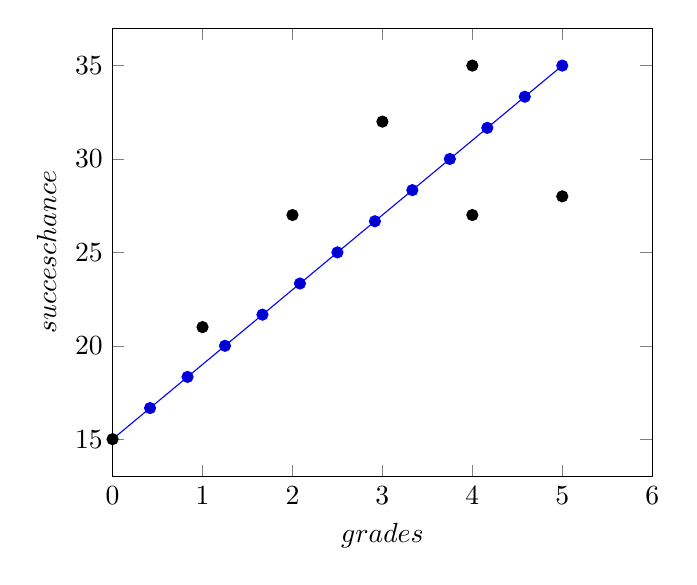
\begin{tikzpicture}
  \begin{axis}[ 
    xlabel=$grades$,
    ylabel={$succes chance$},
    xmin = 0,
	xmax = 6,
  ] 
    \addplot {15 + 4 * x}; 
    \addplot[only marks] coordinates {
		(0, 15)
		(1, 21)
		(2, 27)
		(3, 32)
		(4, 35)
		(5, 28)
		(4, 27)
	};
  \end{axis}
\end{tikzpicture}
\caption{Lineair Regression} \label{fig:regression}
\end{figure}

\noindent The hypothesis is the core of a machine learning algorithm. During the training process, the algorithm learns what the hypothesis looks like. More specifically, it tries to find correct values for the vector $\theta$ (as seen in equation~\ref{hypothesisfunc}. Once the hypothesis has been determined, the difficult work is done. The hypothesis forms the predictive model. The prediction itself is straightforward. A new datapoint is entered into the hypothesis equation and it returns the predicted value.

\subsection{Cost function}
\label{costfunction}
In order to construct a good hypothesis function, good values of $\theta$ have to be chosen. This can be seen as a minimization problem. The difference between any output $y$ and $H_0(x)$ has to be minimized. More concretely, the squared difference has to be minimized. This is the MSE, "Minimum Squared Error" function or also called the cost function. The notation $x^{(i)}$ and $y^{(i)}$ is to denote the $i$th training sample. With dataset size $m$, the MSE is \cite{stanford}:
\begin{align}
J(\theta) = \dfrac{\sum\limits_{i=1}^m(H_0(x^{(i)}) - y^{(i)})^2}{2m} 
\end{align}
\noindent Seeing this equation already makes it clear that the number of training samples is important. From statistics, it is known that the population of data points, in this case training samples, have to be large enough. This problem is addressed later in Section~\ref{overfitting}.

\subsection{Gradient descent}
To solve the minimization problem, the first step is to start with $\theta$ and keep changing the values to minimize $J(\theta)$. This is an iterative approach.  Gradient descent is such an algorithm that can be used to find a solution to the minimization problem. Gradient descent is an algorithm that uses the gradient or derivative of a function to find a local minimum of that function. \\\\
In order to easily explain the gradient descent algorithm, a analogy to a ball rolling down a hill can be made. \cite{rollingBall} Let's say we have a landscape such as in Figure~\ref{fig:gradient}. The horizontal location of the ball represents the values of $\theta$, the height of the ball represents the MSE. We want to get the ball to the lowest possible point, in order to minimize the MSE. To do this, the ball rolls down the hill until it comes to rest at the lowest point. Every iteration of gradient descent will bring the ball closer to the lowest point. \\\\
Of course, when a ball rolls down a hill, it does not just roll down and immediately stop. The ball takes a path similar as described in Figure~\ref{fig:gradient}. When the ball finally comes to rest, it can be said that the algorithm converges to that horizontal position.
 \begin{figure}[H]
\centering
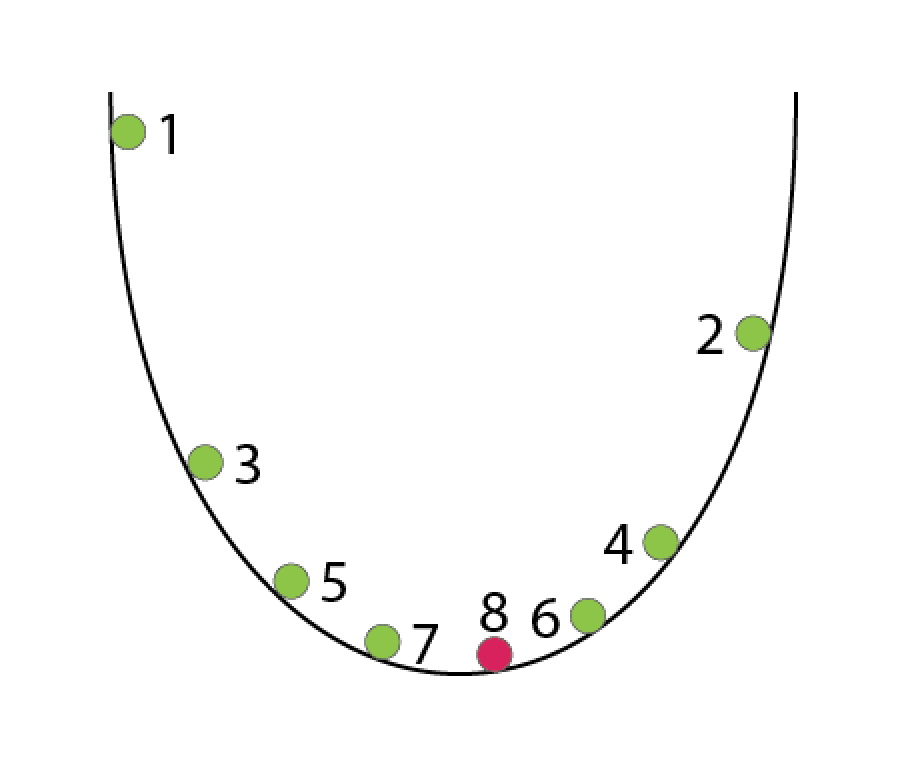
\includegraphics[width=0.7\textwidth]{Figures/gradient}
\decoRule
\caption[Gradient descent]{Iterations of gradient descent. \cite{gradient-fig}}
\label{fig:gradient}
\end{figure}
\noindent A gradient descent algorithm does this using the following algorithm with a simultanious update for all values of $\theta$ \cite{stanford}:
\begin{lstlisting}
            repeat until convergence {
 \end{lstlisting}
\begin{align}
    \theta_j = \theta_j - \alpha\dfrac{\partial}{\partial \theta_j}J(\theta)
\end{align}
\begin{lstlisting}
            }
 \end{lstlisting}
\begin{align}
\dfrac{\partial}{\partial \theta_j}J(\theta) =  \dfrac{\sum\limits_{i=1}^m(H_0(x^{(i)}) - y^{(i)}) * x_j^{(i)}}{m}
 \end{align}
 The equation uses the derivative. A derivative indicates the rate of change, in this case, how steep the hill is. If the hill is very steep, then we move the ball a lot more than when the ground beneath the ball is almost flat.\\\\
 $\alpha$ is the learning rate of the gradient descent. The value of $\alpha$ describes how fast the gradient descent algorithm approaches the local mimimum. If $\alpha$ is too small, the gradient descent can be very slow. In the other case, if $\alpha$ is too large, the gradient descent can overshoot the local mimimum. It may fail to converge and could even diverge. \\\\ 
To go back to the example of the rolling ball, having $\alpha$ too large, could be seen as having the ball roll down the hill extremely fast. Because of this, the ball could come to rest at another point in the landscape, it might have flown over the hill. \\
 \\
The value of $\alpha$ does not need to change during the gradient descent, since the closer the gradient descent gets to the local mimimum, the smaller the derivative becomes, and smaller steps will be taken. If $\theta_j$ is already a local minimum, the derivative is $0$ and the gradient descent will not change the value of $\theta_j$. \cite{courseraLecturesGradient}

\subsection{Normal equation}
There is another method that could be used in place of gradient descent, a normal equation. This is a method to solve for $\theta$ analytically. But this method becomes slow when there are a lot of features. $X$ is a $m$ X $n$ matrix constructed by putting all training samples (vectors of features) together. The notation $x^{(i)}$ and $y^{(i)}$ is used to denote the $i$th training sample. With dataset size is denoted by $m$.
 \begin{gather}
  \theta =  (X^TX)^{-1}X^Ty
  \end{gather}
But what happens when $(X^TX)$ is non-invertible, or singular? This means there are redundant features or more features than training samples. There are mathematical models, such as the pseudo-inverse to still compute a correct result. There are still other methods that could replace gradient descent, such as conjugate gradient, BFGS and L-BFGS. Thinking about matrices and non-invertibility can help to be able to understand how features relate to eachother.

\subsection{Feature scaling}
The main idea behind feature scaling is to make sure that the different features are on a similar scale. The reason behind this is to optimize the gradient descent algorithm. The gradient descent will converge much more quickly with feature scaling. With feature scaling, the partial derivative will be larger and because the features are in scale, the values of $\theta$ will also be similar in scale.\\
\\
When one feature is very large and another is very small, the values of $\theta$ need to be small for the first feature and larger for the second, since the cost function needs to be minimized. This means that the values of $\theta$ need to change more and thus, requires more iterations for the gradient descent algorithm. The range that should approximately be used is $-1 < x < 1$. \\
\\
Mean normalization could be used. This replaces each $x_i$ with $\dfrac{x_i - \mu_i}{s_i}$, where $\mu_i$ is the average value of all $x_i$ values and $s_i$ is the standard deviation.\\
\\
Lets use a numeric example. There are two data points, $(0.5, 3, 1)$ and $(0.7, 4, 2)$ with $(x_1, x_2, y)$. The hypothesis is:
\begin{align}
H_0(x) = \theta_1 * x_1 + \theta_2 * x_2
\end{align}
\noindent In Figure~\ref{fig:costwithscale}, it can be seen that the values of $\theta$ quite quickly fall into the blue zone, where the cost function is minimal. The values of $\theta$ also seem to be equally large when the cost function is minimal. This in contrary to Figure~\ref{fig:costwithoutscale}. Here, both values of $\theta$ need to change a lot. They are not even remotely close to eachother. 

\begin{figure}[H]
\centering
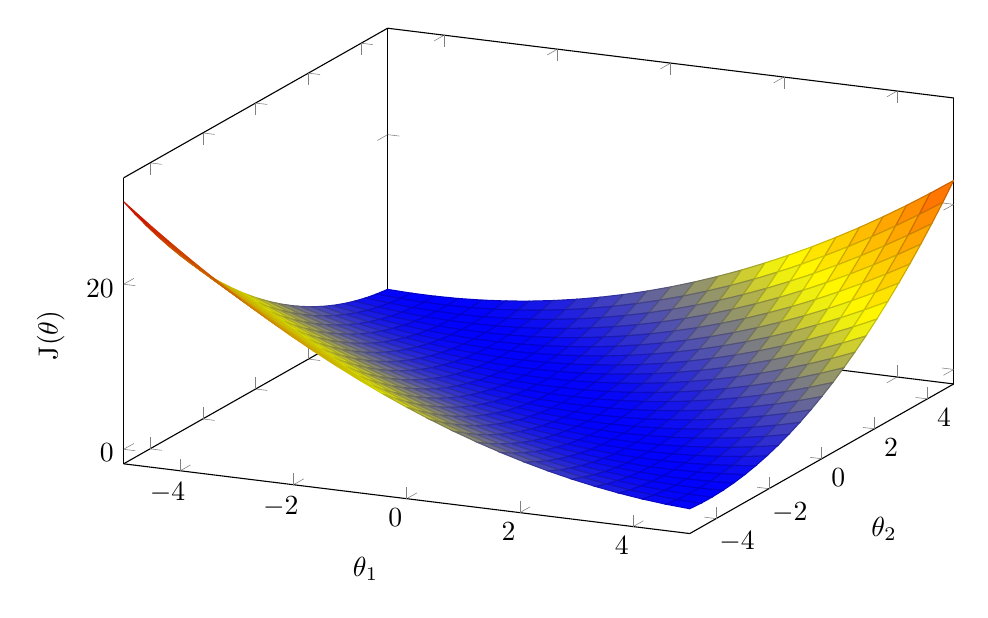
\begin{tikzpicture}
    \begin{axis}[
        width=\textwidth,
        height=8cm,
        xlabel=$\theta_1$,
        ylabel=$\theta_2$,
        zlabel=J($\theta$)]
      % plot the stirling-formulae
      \addplot3[surf] {( (-0.71*x-0.71*y-1)^2 + (0.71*x+0.71*y-2)^2)/(2*2)};
    \end{axis}
\end{tikzpicture}
\caption{Cost function with feature scaling} \label{fig:costwithscale}
\end{figure}

\noindent When $\theta_2$ is near $-4$, the gradient descrent will change $\theta_1$ towards a larger value. However, when $\theta_2$ is near $4$, the gradient descrent will change $\theta_1$ towards a smaller value. In the gradient descent algorithm, $\theta_2$ will converge towards approximatly $-1$ and the actual value of $\theta_2$ will change between being larger and smaller than this value. Because of this, the value of $\theta_1$ takes a longer time to converge.

\begin{figure}[H]
\centering
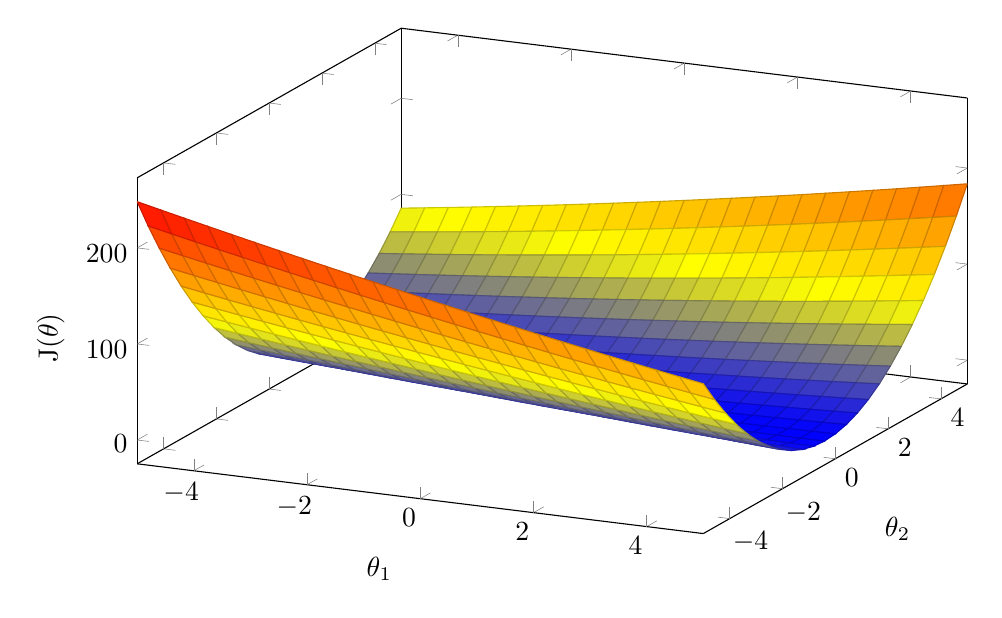
\begin{tikzpicture}
    \begin{axis}[
        width=\textwidth,
        height=8cm,
        xlabel=$\theta_1$,
        ylabel=$\theta_2$,
        zlabel=J($\theta$)]
      % plot the stirling-formulae
      \addplot3[surf] {( (0.5*x+3*y-1)^2 + (0.7*x+4*y-2)^2)/(2*2)};
    \end{axis}
\end{tikzpicture}
\caption{Cost function without feature scaling} \label{fig:costwithoutscale}
\end{figure}

\section{Classification with logistic regression}
\label{classification}
In a classification model, the machine learning algorithm tries to sort data into different classes. The simplest version is binary classification. For example, "is the email spam or not". In lineair regression, the hypothesis can output values other than the classes that exist. However there is a method, logistic regression, which constrains the hypothesis to the available classes.

\begin{figure}[H]
\centering
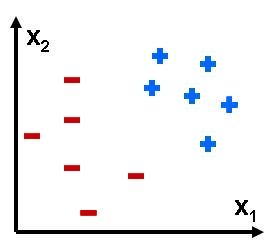
\includegraphics[width=0.5\textwidth]{Figures/binclass}
\decoRule
\caption[Binary classification]{Binary classification. \cite{binclass}}
\label{fig:binclass}
\end{figure}
\noindent Figure~\ref{fig:binclass} shows a simple binary classification example. $x_1$ and $x_2$ are features. Some points belong to the minus class, others belong to the plus class. A logistic regression or classification algorithm will learn from training data what data from the minus class and data from the plus class looks like. Afterwards, the classifier can be used to predict whether an input sample belongs to the minus class or the plus class.

\subsection{Logistic regression}
In logistic regression, a hypothesis is needed which outputs whether an input datapoint belongs to a class or not. It can also be explained as, "what is the chance that the input belongs to a class"? Now the hypothesis needs to output a percentage, the chance that the input belongs to a certain class. \\\\
Then a decision boundary is used. This decides whether the input belongs to the class or not. Usually the decision boundary is $0.5$. If the hypothesis outputs a value higher than the decision boundary, it can be said that the input belongs to the class for which it is being tested. Logistic regresion uses the Sigmoid or logistic function for the hypothesis:
\begin{align}
g(z) =  \dfrac{1}{1 + e^{-z}}
\end{align}
\begin{figure}[H]
\centering
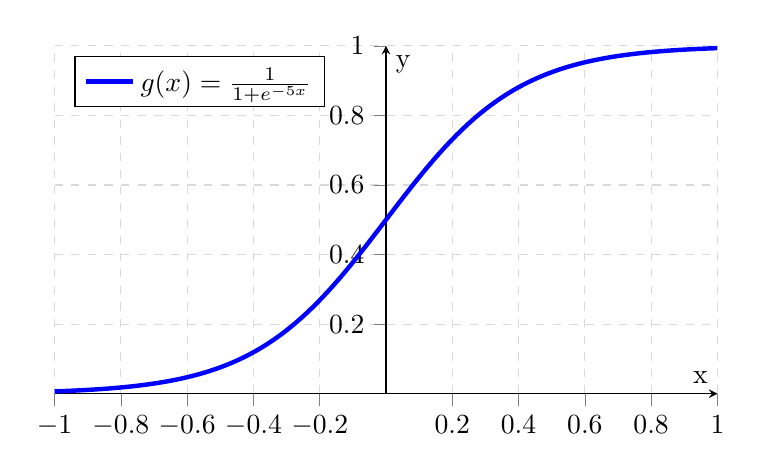
\begin{tikzpicture}
    \begin{axis}[
    	legend pos=north west,
        axis x line=middle,
        axis y line=middle,
        grid = major,
        width=10cm,
        height=6cm,
        grid style={dashed, gray!30},
        xmin=-1,     % start the diagram at this x-coordinate
        xmax= 1,    % end   the diagram at this x-coordinate
        ymin= 0,     % start the diagram at this y-coordinate
        ymax= 1,   % end   the diagram at this y-coordinate
        %axis background/.style={fill=white},
        xlabel=x,
        ylabel=y,
        tick align=outside,
        enlargelimits=false]
      % plot the stirling-formulae
      \addplot[domain=-1:1, blue, ultra thick,samples=500] {1/(1+exp(-5*x))};
      \addlegendentry{$g(x)=\frac{1}{1+e^{-5x}}$}
    \end{axis}
\end{tikzpicture}
\caption{Sigmoid function} \label{fig:logregression}
\end{figure}
\noindent Using this function, the hypothesis can be written as:
\begin{align}
H_0(x) = g(\theta^TX) = \dfrac{1}{1 + e^{\theta^TX}}
\end{align}
\subsection{Cost function}
The cost function from lineair regression cannot simply be applied to logistic regression. For classification it is important that data that belongs to the class has an output closer to 1, and that data that does not belong to the class has an output closer to 0. To do this a different cost function should be used. The notation $x^{(i)}$ and $y^{(i)}$ is used to denote the $i$th training sample. With dataset size is denoted by $m$. A helper function $Cost$ is used. This helps to see the parallel with the cost function for linear regression, as seen in Section~\ref{costfunction}.  \cite{courseraLecturesCost}
\begin{gather}
J(\theta) = \dfrac{\sum\limits_{i=1}^m(Cost(H_\theta(x^{(i)}), y^{(i)}))}{m}\\
  Cost(H_\theta(x^{(i)}), y^{(i)}) =	\begin{cases}
        	 									     - log(H_\theta(x^{(i)})), & \text{if } y^{(i)} = 1\\
        									        - log(1 - H_\theta(x^{(i)})), & \text{if } y^{(i)} = 0\\
            									\end{cases}
\end{gather}
The given cost function accomplishes exactly what is wanted. If the expected output is 1 (belongs to a class), then the cost becomes greater as the output goes to 0 and analogous if the expected output is 0. Gradient descent for logistic regression is exactly the same as for lineair regression except with a different hypothesis. \\
\\
A very simple example of the cost function would be the following. Take one data point, $(3)$ with outputs $1$. The hypothesis seen in Figure~\ref{fig:hyporegresion} and is:
\begin{align}
H_0(x) = \dfrac{1}{1 + \exp{\theta_1 * x_1}}
\end{align}
\noindent The cost function is: $-log(\theta_1 * 3)$ which is graphed in Figure~\ref{fig:costregression} becomes larger when the hypothesis goes towards $0$, and goes to $0$ when the hypothesis goes towards $1$. This is indeed the behaviour that is expected from the cost function for logistic regression.

\begin{figure}[H]
\centering
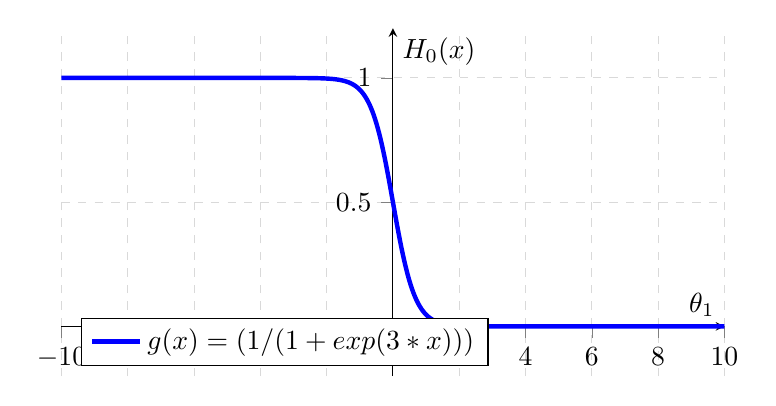
\begin{tikzpicture}
    \begin{axis}[
    	legend pos=south west,
        axis x line=middle,
        axis y line=middle,
        grid = major,
        width=10cm,
        height=6cm,
        grid style={dashed, gray!30},
        xmin=-10,     % start the diagram at this x-coordinate
        xmax= 10,    % end   the diagram at this x-coordinate
        ymin= -0.2,     % start the diagram at this y-coordinate
        ymax=1.2,   % end   the diagram at this y-coordinate
        %axis background/.style={fill=white},
        xlabel=$\theta_1$,
        ylabel=$H_0(x)$,
        tick align=outside,
        enlargelimits=false]
      % plot the stirling-formulae
      \addplot[domain=-10:10, blue, ultra thick,samples=500] {( 1 / (1 +  exp(3 * x) )   )};
      \addlegendentry{$g(x)=( 1 / (1 +  exp(3 * x) )   )$}
    \end{axis}
\end{tikzpicture}
\caption{Hypothesis function example} \label{fig:hyporegresion}
\end{figure}

\begin{figure}[H]
\centering
\begin{tikzpicture}
    \begin{axis}[
    	legend pos=north west,
        axis x line=middle,
        axis y line=middle,
        grid = major,
        width=10cm,
        height=6cm,
        grid style={dashed, gray!30},
        xmin=-0,     % start the diagram at this x-coordinate
        xmax= 1,    % end   the diagram at this x-coordinate
        ymin= -2,     % start the diagram at this y-coordinate
        ymax=6,   % end   the diagram at this y-coordinate
        %axis background/.style={fill=white},
        xlabel=$\dfrac{1}{1 + \exp{3*\theta_1}}$,
        ylabel=$J(\theta)$,
        tick align=outside,
        enlargelimits=false]
      % plot the stirling-formulae
      \addplot[domain=-0:1, blue, ultra thick,samples=500] {-ln(  x )) };
      \addlegendentry{$g(x)=-log(x)$}
    \end{axis}
\end{tikzpicture}
\caption{Cost function example} \label{fig:costregression}
\end{figure}

\subsection{Multi-class classification}
The above hypothesis and cost function are for binary classification. To compute multi-class classification, the One-vs-all algorithm could be used. This algortihm splits the multiples classes into two groups. One group contains one class, the other group contains all other classes. Using these two new groups, the algorithms for binary classification can be used. In other words, for each class $i$ a different logistic regression classifier $H_\theta(x)$ is trained to predict the probability that $y = 1$. On an input x, the most probable class is chosen. \\\\
Another method called One-vs-One could be used. This method compares all pairs of classes. It checks, "does the input belong rather to class A as compared to class B". It does this for all pairs and decides which class most likely contains the input. \\\\
The One-vs-One method uses $n_classes * (n_classes - 1) / 2$ different logistic regression classifier $H_\theta(x)$. Each of these classifiers is trained to fit a pair of classes. \cite{pattern}\\\\
To provide an example, Figure~\ref{fig:multiclass} can be used. On the left, binary classification is shown. The hypothesis and cost function as seen in the above sections can be used to do the classification. On the right, multi-class classification is used. There are three classes: triangles, squares and crosses.
\begin{figure}[H]
\centering
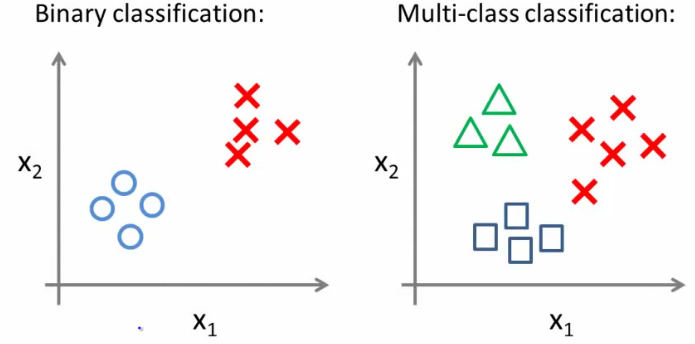
\includegraphics[width=1\textwidth]{Figures/multiclass}
\decoRule
\caption[Multiclass classification]{On the left, binary classification is shown. On the right, three different classes are used. \cite{multiclass}}
\label{fig:multiclass}
\end{figure}
\noindent One-vs-all classification will have to use three classifiers to predict which class a given input sample belongs to. The first classifier predicts whether the input samples belongs to the triangles or to another class. The second classifier predicts whether the input samples belongs to the squares or to another class and analogous for the third classifier. This method can quite quickly find the result. If the first classifier is used first and it is found that the input sample belongs to the triangles class, the prediction is done. \cite{multiclass} \\\\
One-vs-One classification will have to use six classifiers. Each classifier is trained to predict whether an input sample belongs to the triangles or the squares, to the triangles or the crosses, and so on. If the classifiers predict that the input samples belongs rather to the triangle class than to the square class and rather to the triangle class than to the crosses class, it can be predicted that the input sample belongs to the triangle class. Because the One-vs-One classification has to use more classifiers than One-vs-All, it is also slower. However, because it compares all pairs it is also more accurate. \cite{multiclass}

\section{Overfitting}
\label{overfitting}
When the data is not modeled correctly and the model is too precise for the training data, a problem called overfitting occurs. Models that are overfitted have high variance, there are too many possible hypotheses. In other words, if there are too many features, the hypothesis may fit the training set very well but fails too correctly predict new examples. The hypothesis becomes very complex. An example of this can be seen in Figure~\ref{fig:overfitting}. In a similar way, underfitting may occur. 
\begin{figure}[H]
\centering
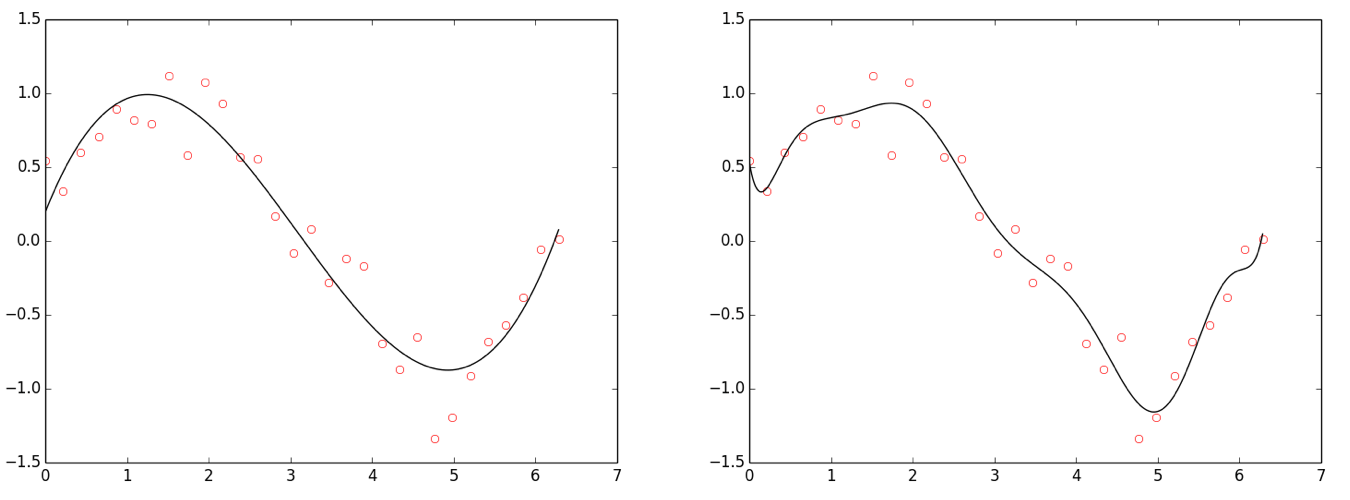
\includegraphics[width=1\textwidth]{Figures/overfit}
\decoRule
\caption[Overfitting]{The points are generated by a sin function with Gaussian noise. Left: good fit (polynomial of degree 3), Right: overfit (polynomial of degree 10). \cite{overfit-fig}}
\label{fig:overfitting}
\end{figure}
\noindent There are methods to avoid overfitting. It is possible to reduce the amount of features.  This can be done manually or by using a model selection algorithm which is explained in Section~\ref{modelselection}. Another option is regularisation. This method keeps all features but manages the values of the parameters of $\theta$.  Regularisation works well when there are a lot of features that all contribute to be able to make correct predictions $y$.\\
\\
A hypothesis is complex when the values of $\theta$ are too large. Regularisation tries to solve this problem. When regularisation is used, the chosen values of $\theta$ become lower. For lineair regression, this can be done in the cost function by redefining the cost function as:
\begin{align}
J(\theta) = \dfrac{\sum\limits_{i=1}^m(H_0(x^{(i)}) - y^{(i)})^2 + \lambda * \sum\limits_{j=1}^m(\theta_j^2)}{2m}
\end{align}
The only change to the cost function is that a penalty is added for large values of $\theta$. When values of $\theta$ become larger, the cost function also becomes larger. When this cost function is minimized lower values for $\theta$ will be chosen. Only $\theta_1$ till $\theta_m$ should be regularised. $\lambda$ is called the regularisation parameter. Because of this small modification, the hypothesis that is constructed will be simpler.
\\\\
Lets use a numeric example. There are two data points, $(3,1)$ and $(5,2)$. The hypothesis is:
\begin{align}
H_0(x) = \theta x_1
\end{align}
\begin{figure}[H]
\centering
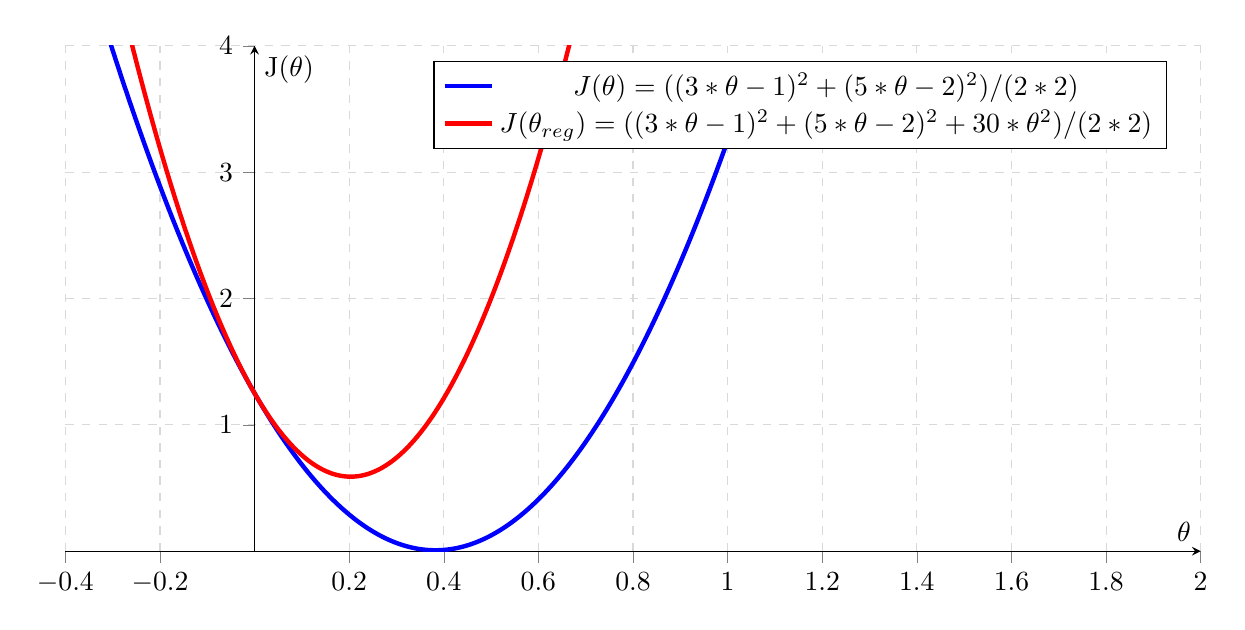
\begin{tikzpicture}
    \begin{axis}[
    	legend pos=north east,
        axis x line=middle,
        axis y line=middle,
        grid = major,
        width=16cm,
        height=8cm,
        grid style={dashed, gray!30},
        xmin=-0.4,     % start the diagram at this x-coordinate
        xmax= 2,    % end   the diagram at this x-coordinate
        ymin= 0,     % start the diagram at this y-coordinate
        ymax= 4,   % end   the diagram at this y-coordinate
        %axis background/.style={fill=white},
        xlabel=$\theta$,
        ylabel=J($\theta$),
        tick align=outside,
        enlargelimits=false]
      % plot the stirling-formulae
      \addplot[domain=-1:1, blue, ultra thick,samples=500] {((3*x-1)^2 + (5*x-2)^2)/(2*2)};
      \addplot[domain=-1:1, red, ultra thick,samples=500] {((3*x-1)^2 + (5*x-2)^2 + 30*x^2)/(2*2)};
      \addlegendentry{$J(\theta)=((3*\theta-1)^2 + (5*\theta-2)^2) / (2*2)$}
      \addlegendentry{$J(\theta_{reg})=((3*\theta-1)^2 + (5*\theta-2)^2 + 30*\theta^2) / (2*2)$}
    \end{axis}
\end{tikzpicture}
\caption{Effect of regularisation} \label{fig:regularisation}
\end{figure}
\noindent In this example, a cost function is constructed with and without regularisation. The blue graph shows the cost function without regularisation, the red graph shows the cost function with regularisation. It can be seen that having regularisation does change the value of $\theta$ where the cost function is minimal, which is exactly what is intended to happen with regularisation. 


\section{Distance metrics}
\label{distancemetric}
Machine learning algorithm also use distance metrics. These can be used to define how to compute distances between different data points that are fed to a machine learning algorithm. There are several different methods to compute distances, both for continuous features and discrete features.  \\
\\
\noindent \textbf{The Euclidean distance} is the distance between two points in the Euclidean space. This can be seen in Figure~\ref{fig:euclideanDistance}. With features $x = (x_1, x_2,..., x_n)$ and $y = (y_1, y_2,..., y_n)$, the Euclidean distance is defined as $\sqrt{\sum_{i=1}^{n}||x_i-y_i||^2}$. When features are continuous, the Euclidean distance is a good metric. However, discrete features cannot be handled by the Euclidean distance. \cite{euclideanDistanceExplain} \\
\\
For example, when a feature represents something such as "country of origin". Countries could be considered continuous. For example the distance between countries could be calculated using \\
$(latitude, longitude)$. In this example, the feature represents the "country of birth" of a person. In that case it does not make sense to use a continuous feature. In this case, the "country of birth" is either equal or not equal. This also shows that a single feature such as a country can be represented as either continuous or discrete depending on the problem that is being solved.\\
\\
Features are almost always represented in numeral methods. "Belgium" could be $1$, "Netherlands" could be $2$, "France" could be $3$, and so on. The difference between "Belgium" and "Netherlands" should be the same as "Belgium" and "France".  \\\\

\begin{figure}[H]
\centering
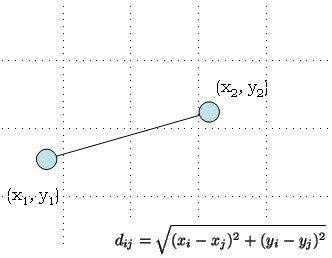
\includegraphics[width=0.6\textwidth]{Figures/euclideanDistance}
\decoRule
\caption[Euclidean Distance]{Euclidean Distance. \cite{euclideanDistance}}
\label{fig:euclideanDistance}
\end{figure}

\noindent \textbf{The Hamming distance} is defined as the number of positions at which the corresponding symbols are different.\cite{hammingDistance} For example, "John" and "Jack" have a Hamming distance of $3$. "Jack" and "Jace" have a Hamming distance of $1$. This can be seen in Figure~\ref{fig:hammingDistance} Going back to the example of countries. Each country can be represented as a number. Each number is seen as a different symbol. For example $10$ is seen as a single number. With the countries, the Hamming distance can only be $0$ (countries are the same) or $1$ (countries are different). \\\\

\begin{figure}[H]
\centering
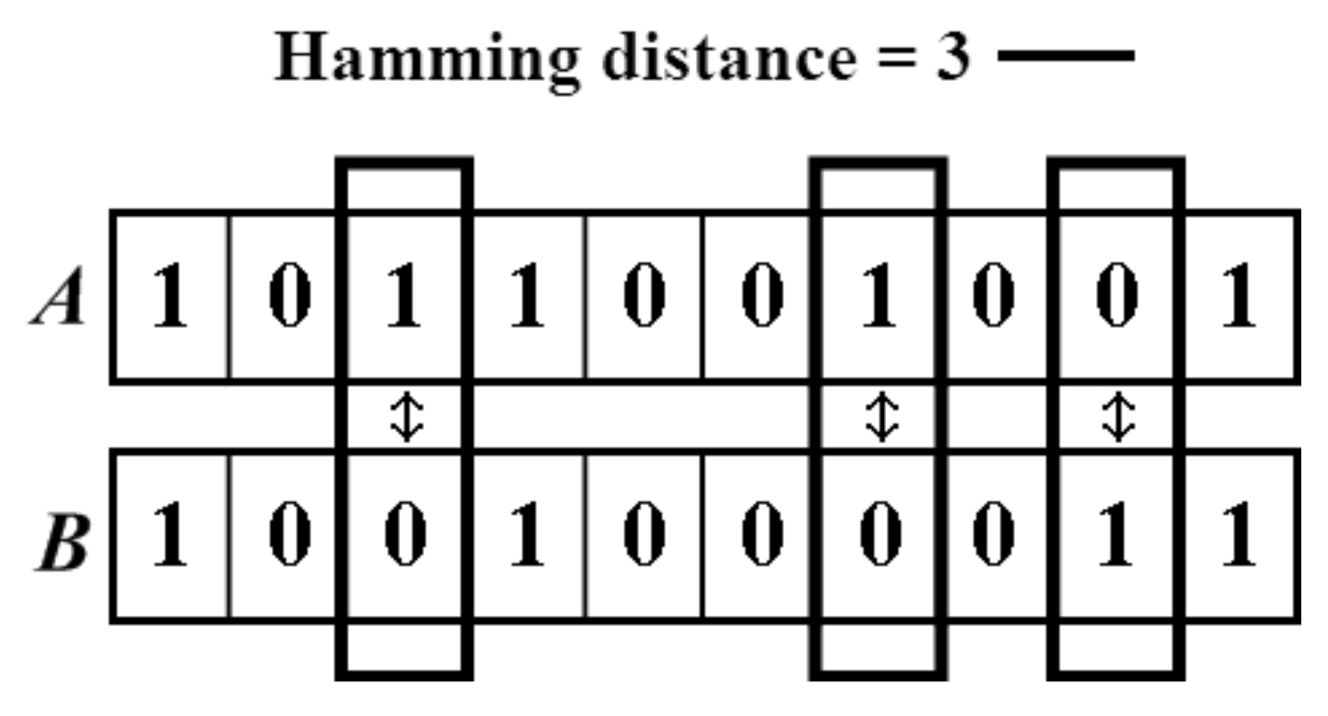
\includegraphics[width=0.6\textwidth]{Figures/hammingDistance}
\decoRule
\caption[Hamming Distance]{Hamming Distance. \cite{hammingDistance}}
\label{fig:hammingDistance}
\end{figure}

\noindent \textbf{The Chebyshev distance} is a distance which is defined as the largest difference between the features. With features $x = (x_1, x_2,..., x_n)$ and $y = (y_1, y_2,..., y_n)$, the Chebyshev distance is defined as \\ $\max_{i=1}(||x_i-y_i||)$. It is also known as chessboard distance. \cite{chebyshevDistanceExplain} It is the amount of moves a king needs to move to another space on a chessboard as seen in Figure~\ref{fig:chebyshevDistance}.  \\\\

\begin{figure}[H]
\centering
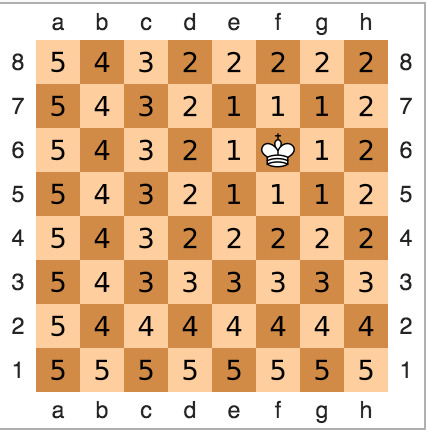
\includegraphics[width=0.6\textwidth]{Figures/chebyshevDistance}
\decoRule
\caption[Chebyshev Distance]{Chebyshev Distance. \cite{chebyshevDistance}}
\label{fig:chebyshevDistance}
\end{figure}

\noindent \textbf{The Manhattan distance} is similar to the Euclidean distance. With features $x = (x_1, x_2,..., x_n)$ and $y = (y_1, y_2,..., y_n)$, the Manhattan distance is defined as $\sum_{i=1}^{n}||x_i-y_i||$. The Manhattan distance is the sum of the difference between each feature. \cite{manhattanDistance} The Manhattan distance in a two-dimensional space is the sum of the difference of the $x$-values and the difference of the $y$-values. An example can be seen in Figure~\ref{fig:manhattanDistance}. \\\\

\begin{figure}[H]
\centering
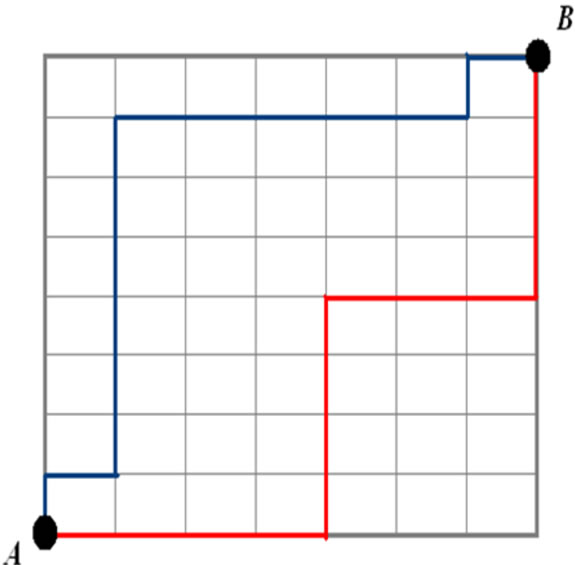
\includegraphics[width=0.6\textwidth]{Figures/manhattanDistance}
\decoRule
\caption[Manhattan Distance]{Manhattan Distance. \cite{manhattanDistance}}
\label{fig:manhattanDistance}
\end{figure}

\noindent \textbf{The Canberra distance} is a weighted version of the Manhattan distance. With features\\ $x = (x_1, x_2,..., x_n)$ and $y = (y_1, y_2,..., y_n)$, the Canberra distance is defined as $\sum_{i=1}^{n}\frac{| x_i - y_i |}{ |x_i| + |y_i|}$. The Canberra distance is the same as the Manhattan distance divided by the sum of the different values. \cite{canberraDistance} \\
\\
\noindent \textbf{The Minkowski distance} is a generalisation of the Euclidean distance and the Manhattan distance. Below the formulas for the Euclidean distance and the Manhattan distance can be seen. However, they are written slightly different. These formulas are almost the same.
\begin{align}
EuclideanDistance(x, y) = (\sum_{i=1}^{n}||x_i-y_i||^2)^{\dfrac{1}{2}} \\
ManhattanDistance(x, y) = (\sum_{i=1}^{n}||x_i-y_i||^1)^{\dfrac{1}{1}}
\end{align}
\noindent A generalisation can be written as: $(\sum_{i=1}^{n}||x_i-y_i||^p)^{\dfrac{1}{p}}$. $p$ is a free variable which can be set. If $p$ goes to infinity, the Chebyshev distance is obtained. The effect of $p$ is shown in Figure~\ref{fig:minkowskiDistance}. This shows that the Minkowski distance is very flexible and powerfull. \cite{minkowskiDistanceExplain} \\\\

\begin{figure}[H]
\centering
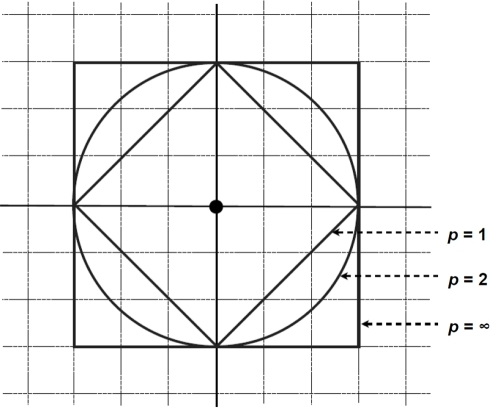
\includegraphics[width=0.6\textwidth]{Figures/minkowskiDistance}
\decoRule
\caption[Minkowski Distance]{Minkowski Distance. \cite{minkowskiDistance}}
\label{fig:minkowskiDistance}
\end{figure}

\noindent The performance of each of these distances on the accuracy depends on the problem that is being solved. Finding the correct distance metric is a matter of trial and error.


\section{Summary}
At the core of a machine learning algorithm is the hypothesis. The hypothesis is the function that is used to fit the training data, it is used to predict values for new data. The hypothesis is constructed using the features that represent the data given to the machine learning algorithm and a set of unknown values $\theta$. \\\\
These values $\theta$ are chosen, as such that the hypothesis is the most accurate. In order to do this, a cost function is constructed. The cost function measures the difference between a known output and a predicted output, usually the MSE is used. The values for $\theta$ can be found by minimizing the cost function. This is done by using the gradient descent algorithm. 
